\chapter{Foundations}\label{foundations}
Most of the groundwork of the methods we will be using was invented in the second half of the 20th century. They include reinforcement learning---a general framework defining the aim of the playing algorithm, Q-learning---a simple algorithm to learn to play a game, and basics of neural networks---the statistical model that was used to overcome Q-learning's limitations.
This foundational work, joined with the recent (after $2010$) advances in the methods of training and architectures of neural networks allowed to vastly improve the former results.

This chapter discusses these methods, as well as describes the Atari machine, as the games we are interested in playing are created for this platform.

\section{Reinforcement learning}
To create an algorithm learning to play a game or solve any other problem, we first have to formally define what the problem is. We will model Atari games within the framework called reinforcement learning. The main property distinguishing reinforcement learning problems from supervised learning (prediction) and unsupervised learning (clustering) is presence of two separate entities: the \emph{environment} and the \emph{agent}.

The environment is the physics or the rules of the game. It presents state, which can be any description of the game, to the agent, scores its action and provides him with the following state.
The agent is the algorithm we prepare. It receives a state it is in from the environment, decides which action to choose there and receives the appropriate reward. Every move happens in a discrete moments of time.

The aim of the creator of the reinforcement learning algorithm is to invent a way to map the game state for each time~$t$: $s_t$ to the action~$a_t$ (possibly storing some inner state), so that the sum:
\begin{equation} \label{discounted-reward}
\sum_{k=0}^{\infty} \gamma^k r_{t + k}
\end{equation}
is maximized. Number $r_T$ is the reward received after doing action~$a_T$ in state~$s_T$. The exponential averaging is called a \emph{discounted} sum, and $0 < \gamma \le 1$ called a \emph{discount factor} corresponds to the level of comfort we have with receiving the awards not now, but in the future. This resembles the way people evaluate their gains---if one is promised a constant amount of money, he'd prefer to receive it rather earlier than later. We assume that every game eventually will find itself in a \emph{terminal} state, which always transitions to a terminal state and gives reward of~$0$. One such progression from the start of the game to reaching a terminal state is called an \emph{episode}.

Both agent and environment are not bound to make their decisions deterministically---in fact, it may be favorable for the agent to play randomly to some extent. In the stochastic case, the aim of the agent is to maximize the discounted sum of expected value of the rewards.

\begin{figure}[!h]
  \center
  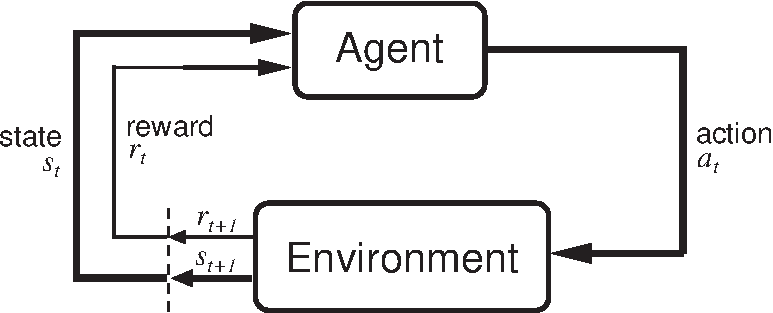
\includegraphics[scale=0.8]{images/Agent-Env-crop.pdf}
  \caption{The interaction between the agent and the environment, from~\cite[Chapter 3.1]{reinforcement-book}.}
\end{figure}

The reinforcement learning, as defined above is a very general framework which can describe a broad range of problems. To make it easier to model it using statistical tools, we assume all the problems we consider are of the form of Markov Decision Process.

Markov~Decision~Process~(MDP) \cite[Chapter 3.6]{reinforcement-book} is a reinforcement learning problem where a distribution of the states and the rewards satisfy Markov property.
\theoremstyle{definition}
\newtheorem{definition}{Definition}
\begin{definition}{Markov property} \label{mdp}
A sequence of random variables $x_i$ satisfies Markov property if and only if the distribution of each variable $x_i$ depends only on the value of the previous variable for all $i$:
  \begin{equation}
    \forall_i\, p(x_i|x_{i-1}, \ldots, x_{0}) = p(x_i | x_{i-1})
  \end{equation}

  In the case of the MDP, Markov property asserts that the distribution of the next states~$s_{t+1}$ and rewards~$r_t$ depends only on the previous state~$s_t$ and the action~$a_t$:

\begin{equation}
\forall_t\, p(s_{t+1}, r_t|s_t, a_t, s_{t-1}, a_{t-1}, \ldots, s_0, a_0) = p(s_{t+1}, r_t|s_t, a_t)
\end{equation}
\end{definition}

This simplifying assumption can be summarized as ``agent has all the information he needs for making actions encoded in the state''. One should note that the representation of the state and not the inner mechanics of environment, is crucial here---imagine a chess player, which sees only bottom half of the board. Even though the game is completely deterministic (assuming deterministic strategy of agent and environment, choosing opponents' moves), agent cannot reliably predict what will be the next state, as there may be pieces on the other part of the board he cannot see yet.

In the case of Atari games played based on the RAM~state, the MDP assumptions are satisfied. The code of the game (saved on ROM), together with a random seed for the game define a deterministic function transforming the RAM (the game state) and awarding rewards.

It is worth noting that the algorithms based on Markov property (TD-learning, Q-learning, Markov Chain Monte Carlo \cite[Chapters 6.1, 6.5 and 5, respectively]{reinforcement-book}) are often used despite the violation of this assumption by the environment. The intuition behind that when the state contains enough information for agent to reasonably approximate the next state and reward distribution, it doesn't matter the approximation will not be accurate. One example of this fact is when we train agents to play Atari games based on the screen state~\cite{nips-dqn}---the player moves influence the inner state (RAM) of the machine, but the changes may not be immediately apparent on the screen. Still, the game screen gives a lot of information about the game state needed to make an action, thus agent can fairly skillfully learn to make good decisions.

\section{Q-learning}\label{qlearning}
Let's call the function (distribution) mapping the current state~$s$ to the action~$a$ chosen by the agent \emph{a~strategy} (or \emph{policy})~$\pi$.

Q-learning~\cite{qlearning} is an algorithm able to choose a strategy in an MDP. It is based on the notion of Q-value: a function mapping the state-action~pair~$(s, a)$, for a fixed strategy~$\pi$, to the expected discounted reward after being in the state~$s$, making an action~$a$ and following the strategy~$\pi$ until the end of the episode.
\begin{equation}\label{q-value}
  Q^\pi(s_t, a_t) = \underset{r\sim p(r_t | s_t, a_t)}{\mathbb{E}} r + \sum_{k=t+1}^\infty \gamma^{k-t}\underset{r\sim p(r_k|s_{k-1}, a_{k-1}), a_k\sim \pi(s_k)}{\mathbb{E}} r
\end{equation}
where $s_k$ is a random variable describing distribution of the states in time~$k$, dependent of the previous state and action, as in equation~\eqref{mdp}. From here on, though, we will assume that choice of the next states and rewards by the environment as well as of actions by the agent are done deterministically---it will simplify the notation and all the statements will hold for the stochastic case when wrapped with the expectation signs. Assuming we store all the state transitions as $next\_state[s, a]$ and the rewards as $reward[s, a]$,\footnote{In the non-deterministic case these can be approximated by, respectively, observed distribution of the next states and the sample averages of rewards in each state-action pair.} the Q-learning algorithm can be written as presented in algorithm \ref{qlearning-pseudo}.

\begin{algorithm} \label{qlearning-pseudo}
  \For{all state-action pairs$ (s, a)$}{
    $Q[s, a] = 0$ \tcp{ initialize Q-values of all state-action pairs}
  }
  \For{all states $s$}{
    $P[s] = random\_action()$ \tcp{ initialize strategy}
  }
  \While{not converged}{
    \For{all states $s$}{
      $P[s] = \argmax_a (R[s, a] + \gamma \max_b(Q[next\_state[s, a], b]))$
    }
    \For{all state-action pairs$ (s, a)$}{
      $Q[s, a] = \alpha(R[s, a] + \gamma \max_b Q[next\_state[s, a], b]) + (1 - \alpha)Q[s, a]$
    }
  }
  \caption{Pseudocode of Q-learning.}
\end{algorithm}

The algorithm makes use of the following property:

\theoremstyle{theorem}
\newtheorem{theorem}{Theorem}
\begin{theorem}\label{qlearning-theorem}
The strategy~$\pi$ is optimal (maximizes the expected discounted reward) if and only if its Q-values satisfy:
\begin{equation}\label{qlearning-property}
  Q^\pi(s_t, a_t) = r_t + \gamma \max_b Q^\pi(s_{t+1}, b)
\end{equation}
for all state-action pairs.
\end{theorem}

Q-learning is a representative of a general domain of algorithms called Generalized Policy Iteration (see~\cite[Chapter~4.6.]{reinforcement-book}). Their approach is to take turns between updating the estimation of the value of the states (in our case Q-values) and updating the strategy to take into account new state value estimation.
 
In the case of Q-learning, the chosen strategy is a greedy one, i.e. it always chooses the action maximizing the immediate reward plus discounted value of the following state:
\begin{equation}
  \pi(s_t) = \argmax_a \big(r(s_t, a) + \max_{a^*} Q^\pi(s_{t+1}, a^*)\big)
\end{equation}
where $r(s, a)$ is the immediate reward after making an action~$a$ in a state~$s$ and~$s_{t+1}$ is (a convenient notation for) a next state after making the action~$a$ in the state~$s_t$.

The update to the Q-values is being made to force more state-action pairs to satisfy the property~\eqref{qlearning-property}:
\begin{equation}
  Q_{new}(s_t, a) := \alpha Q_{old}(s_t, a) + (1 - \alpha)\big(r(s_t, a) + \max_{a^*} Q_{old}(s_{t+1}, a^*)\big)
\end{equation}
$\alpha$ (also called step~size) is a parameter of the algorithm deciding how fast it should move the Q-value estimations toward the ones locally satisfying~\eqref{qlearning-property}. Bigger values lead to faster training, but the convergence proof for constant step~size requires sufficiently small $\alpha$~\cite[section~3.]{qlearning}. It was also shown in~\cite{qlearning-convergence}, that (under the condition that each state-action pair is visited infinitely often) the Q-learning algorithm converges when the variable step~size satisfies:
\begin{equation}
  \sum_t \alpha_t = \infty, \;\;\;\; \sum_t \alpha_t^2 < \infty
\end{equation}


\section{Neural networks}
Many of the current advances in various domains of AI are the effect of improvements of an old\footnote{The predecessor of today's neural network, perceptron, was invented in~$1958$~\cite{perceptron}.} statistical model, inspired by how the brain works: neural network. In this section we define it formally and describe the process of finding best parameters for it.

\subsection{Feedforward neural network}
The simplest neural network, called \emph{feedforward} neural network or \emph{multilayer perceptron} was introduced in~60's~\cite{mlp}.
It consists of a couple of \emph{layers}:\footnote{In the current state-of-the-art models, the number of layers reaches thousands, see e.g.~\cite{stochastic}.} each layer accepts some inputs, processes them, and outputs them as an input for the next layer (see figure~\ref{ann-layers}). The first layer is called input layer, the last---output layer and all the layers in between---hidden layers.
\begin{figure}[h]
  \centering
  \resizebox{0.6\textwidth}{!}{
  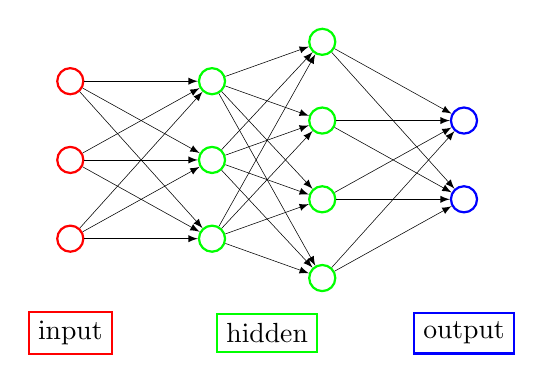
\begin{tikzpicture}

\begin{scope}[very thin]
\foreach \x in {0, ..., 2} {
\node[circle, draw, color=red, thick] (input \x) at (-3, \x) {};
}
\foreach \x in {0, ..., 2} {
  \node[circle, draw, color=green, thick] (hidden1 \x) at (-1.2, \x) {};
  \foreach \y in {0,...,2}
    \draw[-latex] (input \y) -- (hidden1 \x);
}

\foreach \x in {0, ..., 3} {
  \node[circle, draw,color=green, thick] (hidden2 \x) at (0.2, \x-0.5) {};
  \foreach \y in {0, ..., 2}
    \draw[-latex] (hidden1 \y) -- (hidden2 \x);
}

\foreach \x in {0, ..., 1} {
  \node[circle, draw,color=blue, thick] (output \x) at (2, \x +0.5) {};
  \foreach \y in {0, ..., 3}
    \draw[-latex] (hidden2 \y) -- (output \x);
}

\node[rectangle, draw, color=red, text=black, thick] () at (-3, -1.2) {input};
\node[rectangle, draw, color=green, text=black, thick] () at (-.5, -1.2) {hidden};
\node[rectangle, draw, color=blue, text=black, thick]() at (2, -1.2) {output};
\end{scope}
\end{tikzpicture}

  }
  \caption{Architecture of nodes in a feedforward neural network. Each node receives the outputs of the previous layer.}\label{ann-layers} 
\end{figure}

A layer is a composed of \emph{nodes} (also called \emph{neurons}). A node accepts as input the previous layer's nodes' outputs, calculates a linear combination of them and applies a nonlinear function, called \emph{activation} function to the result (see~\ref{ann-nodes}). The typical choices for the activation function are sigmoid: $\frac{1}{1 + e^{-x}}$, hyperbolic tangent, and (popularized recently) rectified linear unit (ReLU): $\max(0, x)$.\footnote{A thorough, yet easy to understand discussion of the various activation functions can be found in~\cite{cs231-actfun}.}
\begin{figure}[h]
  \centering
  \resizebox{0.7\textwidth}{!}{
  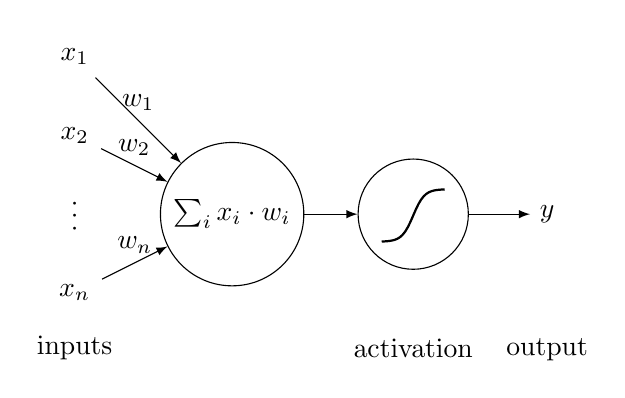
\begin{tikzpicture}[]
\node[circle](x1) at (-2, 2) {$x_1$};
\node[circle](x2) at (-2, 1) {$x_2$};

\node[circle](xn) at (-2, -1) {$x_n$};
\path (x2) -- node[rotate=90]{\ldots} (xn) ;
\node[circle, draw](center) at (0, 0) {$\sum_i x_i \cdot w_i$};
\node[circle, draw, minimum width=1.4cm](activ) at (2.3, 0) {};
\node (output) at (4, 0) {$y$};

\draw[domain=1.9:2.7, thick] plot (\x, {1/(1.5*(1+exp(-14*(\x-2.3)))) - .35});

%\draw[thick] (1.85 , -0.2) --  (2.5, -0.2) -- (2.8, 0.4);

\draw[-latex]  (center) -- (activ);
\draw[-latex] (x1) -- node[above]{$w_1$} (center);
\draw[-latex] (x2) -- node[above]{$w_2$}(center);
\draw[-latex] (xn) -- node[above]{$w_n$}(center);
\draw[-latex] (activ) -- (output);

\node ( ) at (-2,-1.7) {inputs};
\node ( ) at (2.3,-1.7) {activation};
\node ( ) at (4,-1.72) {output};

\end{tikzpicture}

}
  \caption{Details of a neural network node.} \label{ann-nodes}
\end{figure}

The trainable parameters of the model are weights of the linear combination of each of the nodes. The intuition behind introducing multilayer, multinode architecture is that different nodes will learn different statistics useful for producing the output, e.g.~eye or nose detectors for face recognition. The neurons from the earlier layers will learn simple dependencies in the data (e.g.~detection of edges) and the further neurons will combine their information, finding more sophisticated relations (e.g.~dog detector neurons).

\subsection{Gradient descent}\label{gradient descent}
There are a lot of optimization algorithms used to train neural networks, i.e.~find the best set of parameters (weights) for a given network architecture and the data. All of them are a modification of an algorithm of gradient descent \cite{gradient-descent}.

To use it, we first need to choose a loss function, which is a differentiable function of the output of the neural network that correlates with how well the model is doing its job; its value should be high for the bad models and low for the good  models. For example, if we want to predict the depth of each pixel in a photo (useful e.g.~for self-driving cars), we could use a dataset of images accompanied with their depths estimated with a 3D~camera. As a loss function, we could use a mean-squared~error between the real depths and those predicted by the model:
$$
L = \frac{1}{\mbox{\# images}}\sum_{image} \sum_{x, y} (\mbox{real\_depth}(image, x, y) - \mbox{model\_output}(image, x, y))^2
$$

Then, to update the weights of the model to minimize the loss, gradient descent calculates the gradient of the loss with respect to every parameter of the model and moves the weights in the direction of the steepest descent by a small amount~$\varepsilon$, called~\emph{step~size} or \emph{learning~rate}. Choice of a bigger $\varepsilon$ leads to faster learning, but makes the optimization prone to missing good areas of space or diverging completely. Smaller step~size leads to more stable
learning.

The gradients of every weight is determined with the help of chain rule:
\begin{equation}\label{chain rule}
  \frac{\partial}{\partial x} (f \circ g) = (\frac{\partial}{\partial x} f \circ g\big) \cdot \frac{\partial}{\partial x}g
\end{equation}
The equation~\eqref{chain rule} suggests an order of calculating the derivatives: we should first calculate the ones of the weights in the output layer, then previous hidden layer, and so on until the input layer. For example with squared error, sigmoid activation function, datapoints~$x_i$, and target outputs~$y_i$ we have:
\begin{multline}
  \frac{\partial L}{\partial w_{\text{input}, 1}} = \frac{\partial}{\partial w_{\text{input}, 1}} \sum_{i} (y_i - \text{output}(x_i))^2 =\\=  \sum_{i} 2(y_i - \text{output}(x_i)) \cdot \frac{\partial}{\partial w_{\text{input}, 1}}
  ( y_i - \text{sigmoid}(\sum_j w_{\text{output}, j} \cdot \text{hidden}(x_i, j))) =\\=
  \underbrace{\sum_{i} -2(y_i - \text{output}(x_i)) \cdot \text{sigmoid'}(\sum_j w_{\text{output}, j} \cdot \text{hidden}(x_i, j)) \cdot \sum_j \text{hidden}(x_i, j)}_{\sum_j \frac{\partial L}{\partial w_{\text{output}, j}}} \cdot \frac{\partial}{\partial w_{\text{input}, 1}}\ldots
\end{multline}

Because the process of gradient calculation proceeds from the end of the network toward the beginning, it is called \emph{backpropagation} or \emph{backward~pass} (in contrast to \emph{forward} pass, when the network is evaluating outputs).

The calculation of a full loss, based on all examples can be infeasible: current datasets often consist of tens of gigabytes of data (see e.g.~COCO challenge dataset:~\cite{coco-dataset}) and to train a network it is often needed to make a couple of thousands of parameter updates.
To speed the process up, it is common to approximate the full loss function (thus the gradients, too) by a loss calculated on a random subset of data examples. More often than not, a random subset of $100$~examples will possess statistical properties indistinguishable from the whole dataset, leading to accurate (and fast to obtain) estimates of gradients. This process is called \emph{minibatch} training (and the whole algorithm a \emph{stochastic}~gradient~descent) and the size of the \emph{batch} is another hyperparameter of the model. There is a trade-off in its choice---bigger batch size gives better gradient estimates, but takes longer to calculate.

The role of nodes in a neural network is symmetric---there's no reason a particular neuron should behave differently than its neighbor. To enforce neurons to learn various aspects of the data, we initialize the weights randomly. The experiments show that it suffices to make different neurons learn different weights---intuitively, the model with different neurons will have easier time predicting output, as it will be combining various types of information.

One can summarize this section by presenting a stochastic gradient descent pseudocode in algorithm~\ref{sgd-pseudo}. An example implementation for a toy problem can be found in file \texttt{code/gradient-descent.ipynb} on the CD.

\begin{algorithm} \label{sgd-pseudo}
  initialize all weights randomly\;
  \While{\text{not converged \& not exceeded maximum number of iterations}} {
    pick a random subset $S$ of data examples\;
    calculate the loss function for the examples in $S$ in forward pass\;
    calculate the gradients of the loss and update each weight in a backward pass:
    $w := w - \varepsilon \cdot \frac{\partial L}{\partial w}$
  }
  \caption{Pseudocode of gradient descent.}
\end{algorithm}

\section{Deep Learning}
The neural networks were not often applied in modelling until recently. There was a number of factors which contributed to their current successes. In this section we describe shortly the most important of them.

\subsection{Computing power}
Creating good prediction or classification models requires a lot of computation power.\footnote{Deep learning community jokes that the time to train a state-of-the-art model stays a week, regardless of the increase in the computing power.} Neural networks, with their big expression power can provide good results, but only when supplied with enough data. When we pass a little data to a deep neural network, we can often see an \emph{overfitting} effect---the model performs well on the data it saw (training data), but generalizes poorly to unseen examples (test data).

In a world with limited computation power, best results will be biased towards simpler models, like linear regression, random forest, or support vector machines. Out of the whole continuum of~$R^n \rightarrow R^m$ functions, elementary models will pick a small subset of smooth, easy, reasonable ones and will pick the best one with the use of limited data. As the subset of functions that can be expressed is small, they are quite different from each other and it is easy for the model to pick the best function.

When a more involved model is trained, it can represent more functions, but at the expense that it requires more data (thus more computation power). When faced with data scarcity, it doesn't choose the best function among all that it can represent---it falsely detects noise in the data as significant patterns and erroneously treats insufficiently often occurring patterns as noise.

Fortunately, thanks to game industry, we saw a rapid increase in computation speed and memory bandwidth of graphics processing units (see figure~\ref{nvidia-speed}). Most of the current state-of-the-art algorithms for finding best parameters for a neural network can be defined in terms of common matrix operations. Due to sophisticated library implementations and good parallelization properties, these operations can be computed fast using a GPU, leading to efficient training of neural networks. While we saw vast speedups moving from a high-end CPU to a middle range GPU, it is fair to mention that some of the algorithms, e.g. actor-critic methods described in \cite{a3c}, do not experience significant improvement in training time on a GPU in comparison to a CPU.

\begin{figure}[h]
  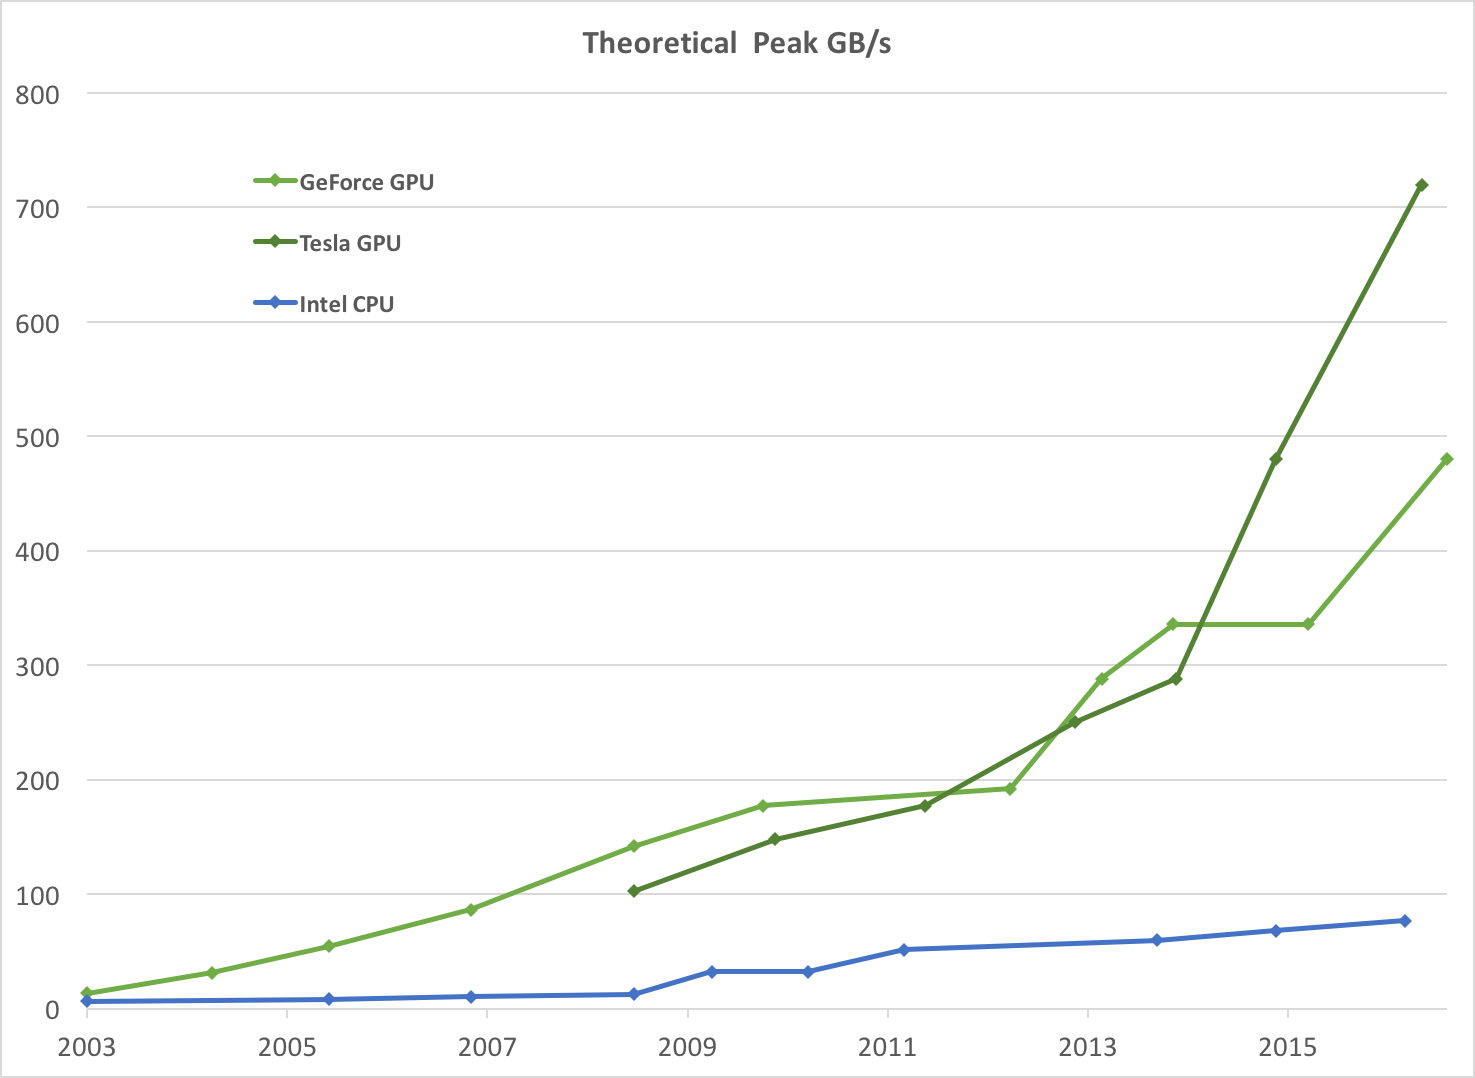
\includegraphics[width=\linewidth]{images/gpu-bandwidth.png}
  \caption{Comparison of best CPU and GPU memory bandwidths in time. Note that the memory bandwidth often constraints the speed of neural network training. Plot comes from \cite{nvidia-docs}.}\label{nvidia-speed}
\end{figure}

\subsection{Better training algorithms}
The speed of convergence of vanilla stochastic gradient descent can be improved in many cases. For example, if the optimization space is a valley with high hills and a river with a little slope in the bottom, SGD will zigzag from one wall of the valley to the other, due to higher gradients between the walls than in the river.

There are a lot of improvements of the SGD to faster move in the optimization space in the situations like this. They include momentum~\cite{momentum}, Adam~\cite{adam}, or Adadelta~\cite{adadelta}. I will describe RMSProp~\cite{rmsprop}, the algorithm that we use in our code. One can read about the others in~\cite[chapter 8.3.]{dlbook} in detail.

\subsubsection{RMSProp}\label{rmsprop-section}
The basic idea of RMSProp is to (pointwise) divide the gradient by the square root of the sum of previous gradients' squares. This way the directions which keep having high gradients in the course of training, will be scaled more and more and directions will low gradients will be more and more ``preferred'' to traverse along.

To prevent vanishing the learning rate too much and significantly slowing down the learning near the end, instead of calculating the sum, RMSProp stores the exponential average of the history of gradients' squares.

The pseudocode of RMSProp can be found in algorithm~\ref{rmsprop-pseudo}.
\begin{algorithm}
  \DontPrintSemicolon
  \SetKwInOut{Input}{input}
  \Input{Initial parameters $\theta$, learning rate $\varepsilon$, decay rate $\rho$, small constant $\delta$ for numerical stability}
  Initialize gradient accumulation $r \leftarrow 0$\;
  \While{not converged}{
    Pick a random subset $S$ of data examples\;
    Calculate gradient: $g \leftarrow \nabla_\theta \sum_{(x, y)\in S} L(f(x, \theta), y)$\;
    Accumulate squared gradient: $r \leftarrow \rho r + (1-\rho) g \cdot g$ (pointwise multiplication)\;
    Compute parameter update: $\Delta\theta \leftarrow \frac{-\varepsilon}{\sqrt{\delta + r}} \cdot g$ (pointwise multiplication)\;
    Update parameters: $\theta \leftarrow \theta + \Delta \theta$\;
  }
  \caption{Pseudocode of RMSProp, adapted from~\cite[Chapter 8.5.2]{dlbook}.}\label{rmsprop-pseudo}
\end{algorithm}

\subsection{Convenient libraries}
Another factor causing deep learning models to rise is the creation of open source libraries for symbolic computation. A mere $6$~years~ago, if a student or a scientist wanted to experiment with neural network models, he had to implement the neural network as a couple of matrix multiplications, calculate the gradients on paper and backpropagate them in code, and implement a version of gradient descent. Not to mention that performing the computation on GPU using a direct memory manipulation library like CUDA significantly increased the code complexity.

Fortunately, around~$2010$ open source libraries, greatly simplifying the process of implementing deep learning models, started to appear. Currently there are $3$~such frameworks which are popular: Theano, Torch and Tensorflow.

Theano~\cite{theano} is a python library developed by Montreal Institute for Learning Algorithms, which the author made a humble contribution to.\footnote{The contribution can be accessed in~\cite{theano-contrib} and contains possibility of evaluation just a subset of outputs of an already compiled Theano function.}

Torch~\cite{torch} is a library allowing to write neural networks in Lua, used and developed by Facebook.

Tensorflow~\cite{tensorflow} is a library made by Google, supporting writing in C\texttt{++} and python. It was the first to seamlessly allow the distributed training of models.

The ideas behind these libraries are similar. All of them allow the user to write the high-level code that will be interpreted as a symbolic computation forming a directed acyclic graph. Then, during execution, it is compiled to a low-level code able to run on a GPU. The libraries decide on the order of calculating the nodes in the graph (called~\emph{Op}s).

Treating the code written by the user as symbolic expressions and deferring its evaluation allow to perform low-level optimization (like in compilers---in a sense these libraries \textit{are} compilers), symbolically calculate the gradient of an expression, and allow for different backends (CPU~vs.~GPU).

\renewcommand{\figurename}{Snippet}
You can see a short example of Theano code in snippet~\ref{theano-code}, which is also available as \texttt{code/theano.ipynb} on the CD.

\begin{figure}[!h]
\begin{Verbatim}[commandchars=\\\{\}]
{\color{incolor}In [{\color{incolor}1}]:} \PY{k+kn}{import} \PY{n+nn}{theano}
        
        \PY{n}{x} \PY{o}{=} \PY{n}{theano}\PY{o}{.}\PY{n}{tensor}\PY{o}{.}\PY{n}{dscalar}\PY{p}{(}\PY{l+s+s2}{\PYZdq{}}\PY{l+s+s2}{x}\PY{l+s+s2}{\PYZdq{}}\PY{p}{)}
        \PY{n}{y} \PY{o}{=} \PY{l+m+mi}{3} \PY{o}{*} \PY{n}{x} \PY{o}{\PYZhy{}} \PY{n}{x} \PY{o}{*} \PY{n}{x}
        \PY{n}{dy} \PY{o}{=} \PY{n}{theano}\PY{o}{.}\PY{n}{tensor}\PY{o}{.}\PY{n}{grad}\PY{p}{(}\PY{n}{y}\PY{p}{,} \PY{p}{[}\PY{n}{x}\PY{p}{]}\PY{p}{)}\PY{p}{[}\PY{l+m+mi}{0}\PY{p}{]} \PY{c+c1}{\PYZsh{} \PYZhy{}2x + 3}
        \PY{n}{f} \PY{o}{=} \PY{n}{theano}\PY{o}{.}\PY{n}{function}\PY{p}{(}\PY{n}{inputs}\PY{o}{=}\PY{p}{[}\PY{n}{x}\PY{p}{]}\PY{p}{,} \PY{n}{outputs}\PY{o}{=}\PY{p}{[}\PY{n}{y}\PY{p}{,} \PY{n}{dy}\PY{p}{]}\PY{p}{)}
        \PY{n}{f}\PY{p}{(}\PY{l+m+mi}{3}\PY{p}{)}
\end{Verbatim}

            \begin{Verbatim}[commandchars=\\\{\}]
{\color{outcolor}Out[{\color{outcolor}1}]:} [array(0.0), array(-3.0)]
\end{Verbatim}
              \cprotect\caption{Example Theano code}
              \label{theano-code}
\end{figure}

\renewcommand{\figurename}{Figure}
Theano, Torch and Tensorflow in their basic form are libraries to express any kind of computation. The popularization of them fueled the creation of many higher level frameworks, even further simplifying implementation of deep models. These libraries, including Keras~\cite{keras}, blocks~\cite{blocks} and TFLearn~\cite{tflearn} allow for implementing typical transformations, like an all connected layer, softmax, or popular activation functions, in one line. They make it easier to read the data, visualize the learning process, and implement the popular optimization algorithms.

\section{Atari~2600}
Atari~2600~\cite{atari} is a game console created in the late 70s. It has a processor running at around~$1$~MHz, mere $128$~bytes of RAM~memory and a joystick with $18$~actions ($9$~positions $\times \{\mbox{fire}, \mbox{no-fire}\}$). To play a game, one needs to insert a cartridge with a ROM of a game (of size $4kB$) and connect the console to the TV~screen. It was producing a new game screen with frequency~$60$Hz using some tricks,\footnote{Interested reader can read a short article about ``racing the beam'' in~\cite{racing-beam}.} needed to show the full image when the RAM fitted only a line of it. A picture of the Atari~2600 can be seen in figure~\ref{atari-picture}.

\begin{figure}
  \centering
  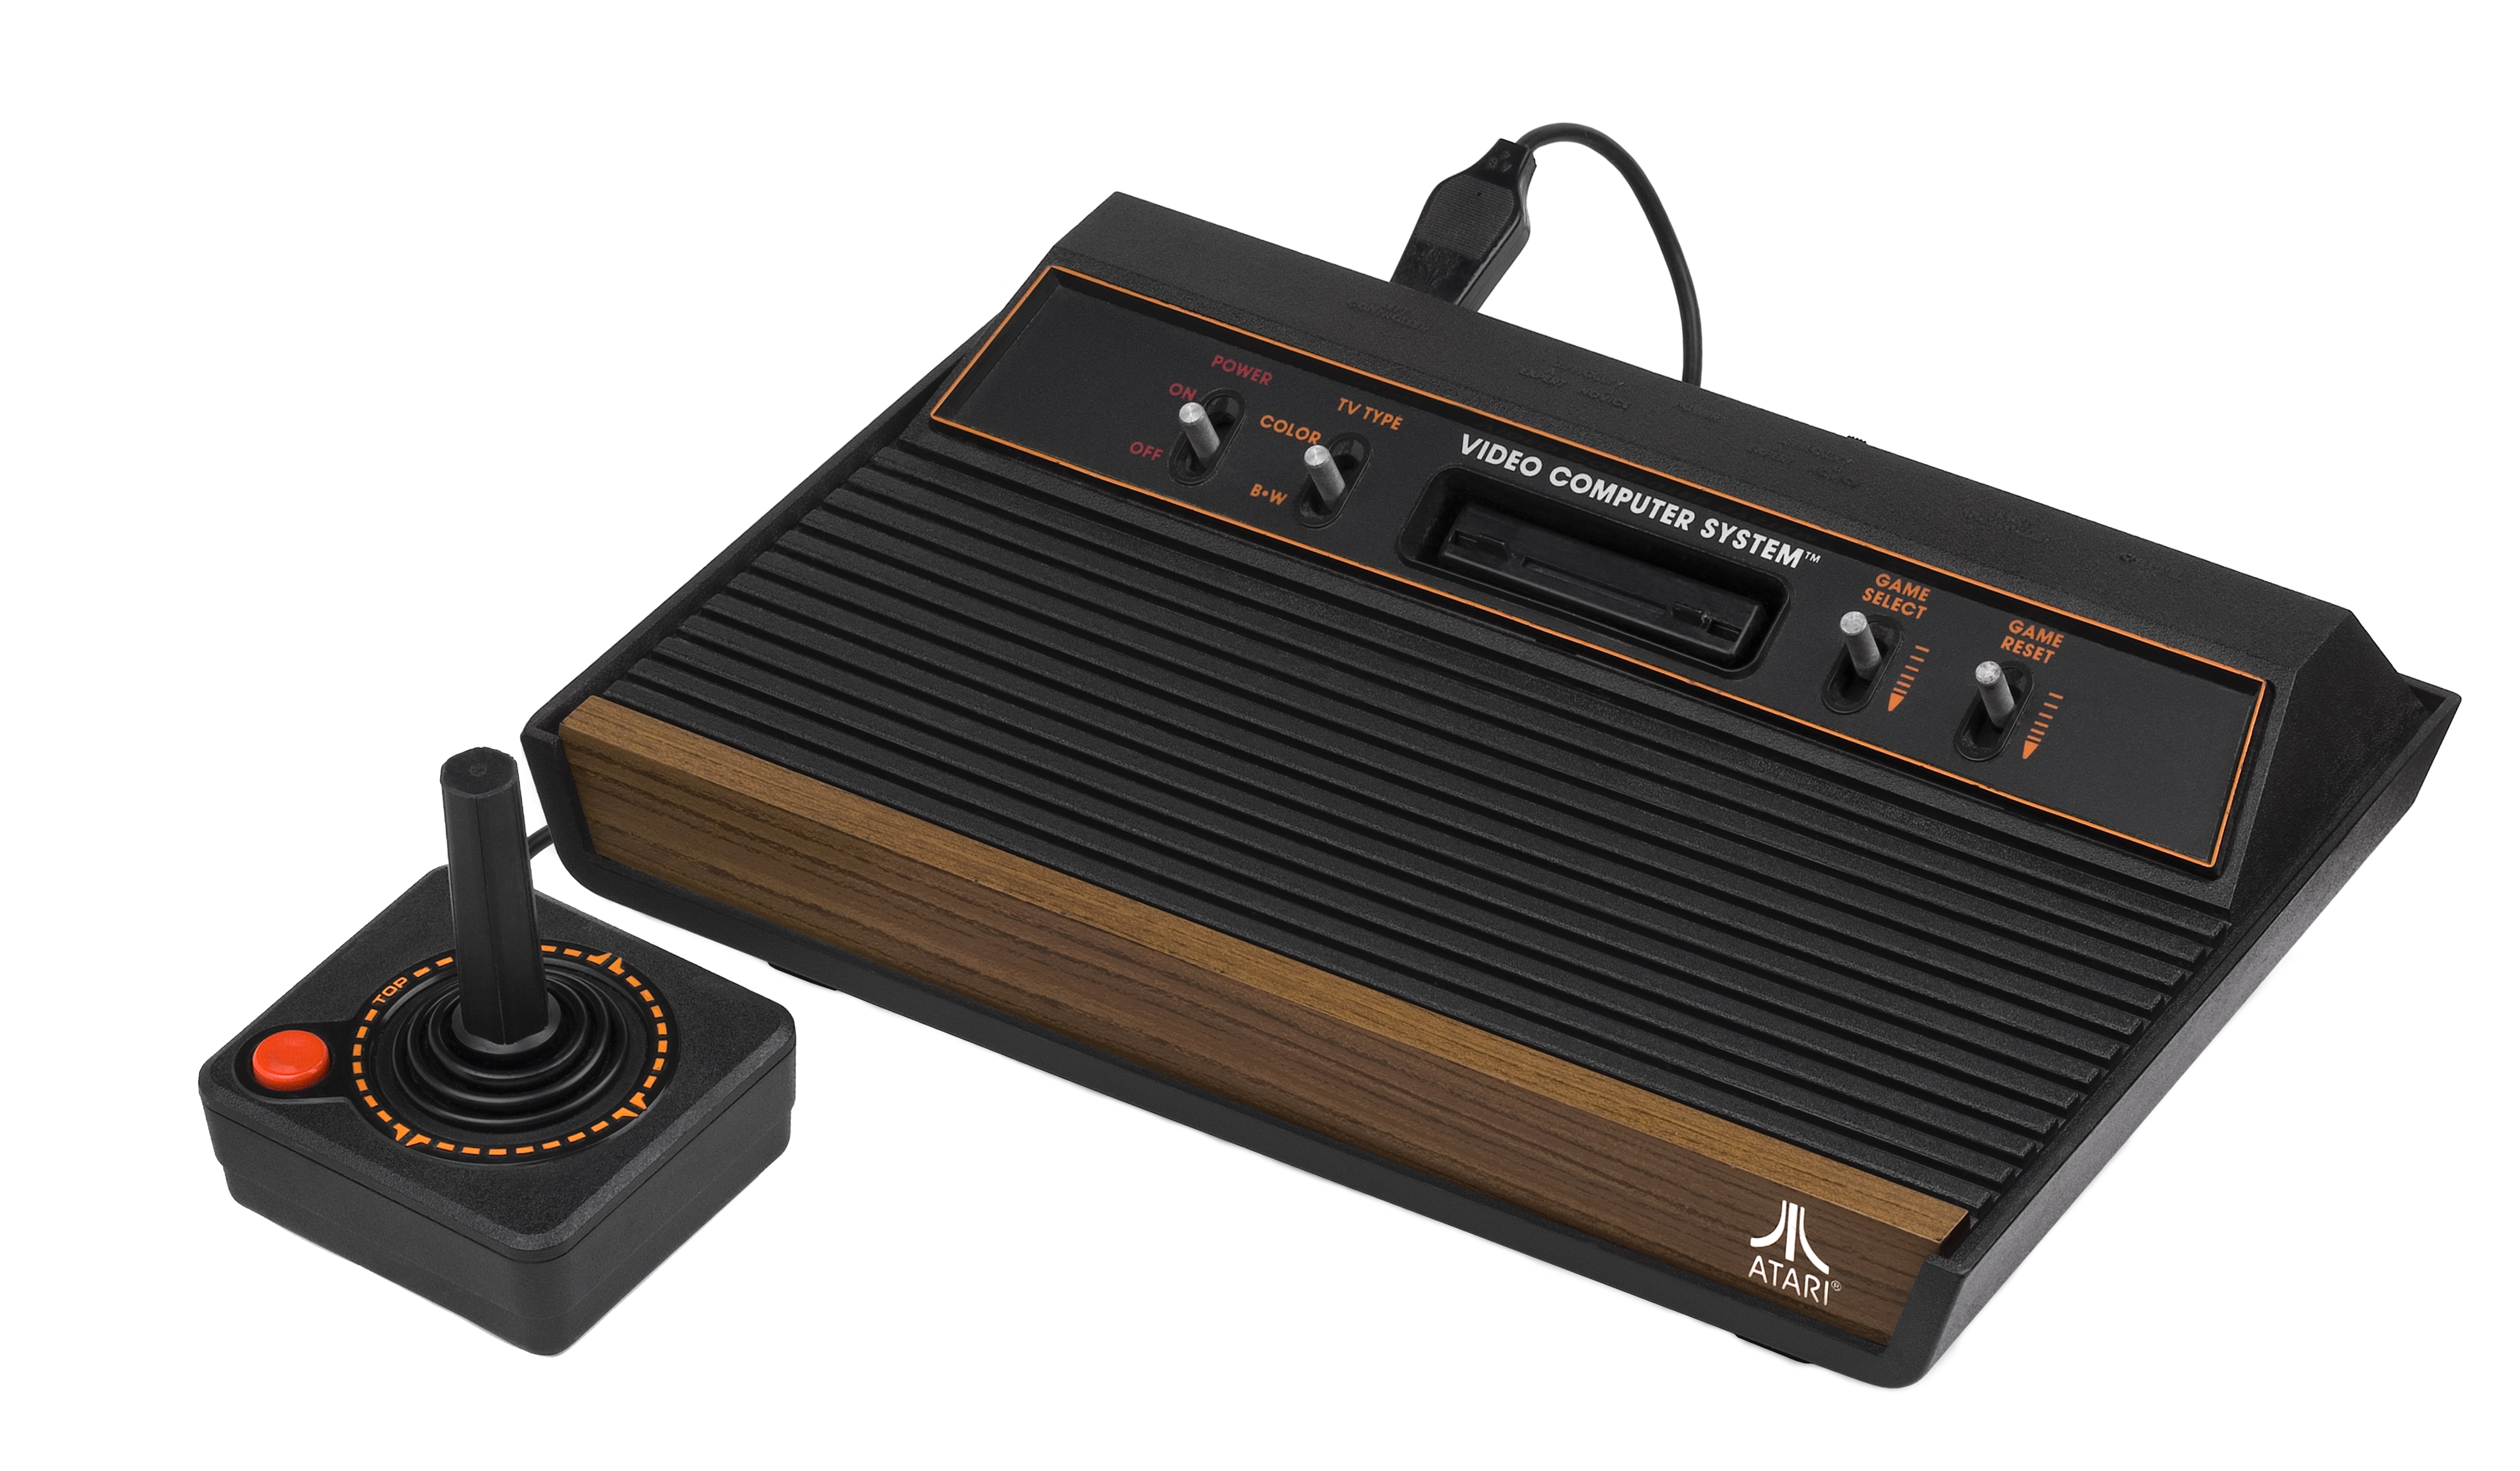
\includegraphics[width=.8\linewidth]{images/atari.jpg}
  \caption{Picture of the Atari machine.}\label{atari-picture}
\end{figure}

The interest in Atari within AI community arose after the publication of~\cite{ale}. It introduces Arcade Learning Environment, a framework which allows for easy creation and evaluation of agents playing Atari games. It encompasses Stella~\cite{stella}, the Atari~simulator for computers. Thanks to~ALE, the programmer can read the screen as a python array, know which actions are possible in each game and read rewards without the need to parse them from the screen nor understanding the details of RAM~memory of each game.

Some time after the release of~ALE, OpenAI, an emerging player in AI, created a convenient wrapper on top of it: OpenAI~Gym~\cite{gym}. It further simplifies the evaluation of the agents, introduces some new, non-Atari environments to test the agents, and make it possible to visualize the training on OpenAI~page, encouraging scientists to open source their ideas.

The diversity of Atari games made it a good challenge for AI agents. There are both very simple games, like Pong, where a good initial position of the paddle can guarantee winning and very involved ones, like Montezuma's~Revenge requiring to collect items and use them correctly.\footnote{The best to our knowledge method for Montezuma's~Revenge~\cite{hdqn}, requires manual formulation of the game's objects and sub-goals, what makes it hardly transferable to other environments.} The work on creating agents capable to play many of the Atari games well resulted in many breakthroughs in AI, including winning the Go game with a human world-champion~\cite{alphago} and creation of deep~Q-learning, to which the next chapter is dedicated.
